% Chapter 1

\chapter{Introduction} % Main chapter title

\label{Chapter1} % For referencing the chapter elsewhere, use \ref{Chapter1} 

\lhead{Chapter 1. \emph{Intro.}} % This is for the header on each page - perhaps a shortened title

%----------------------------------------------------------------------------------------

%Where the genome project mapped the genetic structure of complicated organisms such as the mouse, those pursuing the \textit{neurome} are seeking the same for the neural anatomy. In the recent years, due to the significant progress in biology and imaging techniques, this daunting challenge which forms the first step in understanding the brain appears achievable. In fact, with the considerable amount of image data readily available using modern imaging techniques, the onus is on the signal and image processing community to contribute towards the computational and analytical aspects of the problem. In fact, informatics, not bioimaging or biology itself, remains as the major roadblock in creating a neurome for complex organisms.  

%Modern imaging systems have enabled a new kind of discovery in cellular and developmental biology. With spatial resolutions running from millimeters to nanometers, analysis of cell and molecular structure and dynamics is now routinely possible across a range of biological systems. The development of fluorescent reporters, most notably in the form of genetically encoded fluorescent proteins (FPs) combined with increasingly sophisticated imaging systems enable direct study of molecular structure and dynamics 

%
%The past few years have witnessed significant progress in biological and biomedical imaging techniques, and as a result, image based studies of biological processes have gained significant momentum. 

Recent years have witnessed an increasing trend in collaborative research between the field of biological sciences and engineering. In particular, advances in modern day imaging techniques have enabled biologists to image cellular and subcellular structures over a vast range of spatial resolution, ranging from micrometer to nanometer scale.  Using state of the art imaging protocols, biologists are now able to generate image data at an unprecedented scale. However, while imaging is no longer considered a bottleneck for experimental biology, the sheer volume of data being collected calls for automated processing for high throughput study in cell biology. This has established a new field of interdisciplinary  research -- \textit{Bioimage Informatics} \cite{peng2008bioimage}, leading to a number of cross disciplinary publications as well as software suits for image processing techniques which are specialized for such biological tasks \cite{icy,schindelin2012fiji,schneider2012nih}.


\section{Neuroimage analysis}
A subcategory of the aforementioned  discipline of bioimage informatics involves image analysis for neuroscience. Researchers in this field of \textit{Neuroimage analysis}  borrow techniques from digital image analysis and computer vision for deeper understanding of the brain's functionality (for a model organism) through image based studies.

Functions of an animal's brain are largely governed by its neurons, and the number of neurons vary between a few hundreds in the roundworm \textit{C. elegans}\cite{cElegans} to a hundred billion in an adult human brain. The relationship between the morphology and functionality of neurons was established by Ramon Y Cajal in the 19th century. Cajal’s hypothesis serves as the basis for modern day neuroimage analysis. Studies based on morphological properties of individual neurons and neuronal components such as dendritic spines, synapses, mitochondria etc. have shown promise in better understanding and diagnosis of various neurological disorders and neuro-degenerative diseases \cite{bio_belichenko1994rett,neuron_structure,barry_serotonergic,barry_branching,cuntz_neuron}. It is evident that neuroimage analysis becomes a big data problem as we prepare ourselves to study the nervous system of vertebrates. This suggests that the prevalent norm of data interpretation by a trained human personnel needs to be replaced with sophisticated automation. It is not surprising that this problem has been receiving significant attention over the last few years. For example, the publicly accessible website \textit{neuromorpho.org} \cite{neuromorpho} was published in 2006 with only a few hundreds of neurons in its repository. As of June 2015, neuromorpho.org contains more than ten thousand digitally reconstructed neurons, contributed by researchers from over 120 laboratories worldwide \cite{nanda2015doubling}.


Two basic steps are involved in designing a platform for image based study of the brain -- image acquisition and image analysis \cite{meijering_survey}. 

\subsection{Image Acquisition}
Choice of a particular imaging modality depends on the specific application. Fluorescence microscopy is a popular choice when the study involves a global structural analysis of the neurons or some neuronal components in the micrometer scale. For such imaging techniques, the specimen is genetically tagged with a fluorescence protein (GFP, YFP etc.) which emits photons when illuminated by a light source \cite{barry_branching}. These photons are eventually detected by a sensor to produce a digital image of an optical plane. Laser scanning confocal microscopes are commonly used for fast three dimensional imaging of neurons of model animals such as Drosophila, rat, mice etc. Depending on the application, other imaging techniques such as bright-field microscopy \cite{oberlaender2007transmitted}, multiphoton microscopy \cite{santamaria2007automatic} etc. are also used to image neuronal structures.   Electron microscopy (EM) is a popular choice for imaging neuronal structures at nanometer scale. EM is particularly useful in analyzing subcellular objects and surrounding structures such as mitochondria, synapse, vesicles etc. 

\subsection{Image analysis}
While we are still far away from achieving our end goal of understanding the brain, recent research suggest that detection and quantification of morphological anomalies of certain neuronal structures can answer some relevant questions related to diagnosis of certain neural disorders. Specifically, morphological structure of individual neurons, dendritic spines and certain characteristics of subcellular objects such as synapses, mitochondria etc. reveal important information regarding the brain’s functioning. Anomaly quantification can be performed via comparison of the shape of the objects, which in turn requires a robust segmentation technique. Broadly, the relevant research in neuroimage analysis can be categorized into the following groups: segmentation and shape analysis of individual neurons \cite{dima_wavalet,mukherjee_T2T_2,mukherjee_TuFF,rodriguez_voxelscoop,peng_GAD}, study of the types of dendritic cells and characteristics of the intra neuronal structures\cite{5613939,6008641,6971126,EMmembrane_nguyen}. While the end goal remains the same, all these methods differ considerably from the engineering point of view and require different imaging modalities. As a result, the processing algorithms differ considerably in nature, thus making each of these techniques individual topic of extensive research.

\section{Problem formulation}
In the recent years there have been concerted efforts to develop analytic models for global morphological comparisons of neurons \cite{meijering_survey}. This is because anatomical distortion of neurons provide initial clues toward neurological disease understanding, diagnosis or  monitoring. 
This refers to the branch of study where the geometric and morphological properties of single neuron cells are studied for better understanding of its functioning. Since it is widely believed that structural anomaly of neurons correlate well with changes in its functioning, such global morphological assessments are essential for performing  tasks such as quantification of the neuron degeneration due to a disease or drug usage, identifying young and adult neurons in the brain, differentiating between cells in different layers of the brain etc. \cite{vaccari2012assessment,neuron_structure,cuntz_neuron,barry_branching,barry_serotonergic,bio_belichenko1994rett}.

Designing a workflow for  the aforementioned global shape based study involves two critical steps. First, a digital reconstruction should be obtained from the raw image data. This is the segmentation or tracing stage. Automated algorithms for performing high throughput digital reconstruction is crucial in developing building the neuronal atlas for a species. Till date, such an atlas exists for the round worm \textit{C. elegans} \cite{cElegans}, where the neurons exhibit significantly simpler structural patterns. However, for developed species such as the fruit fly, mice, zebrafish, huumans, \textit{etc.} developing such shape based neuron atlas is still an unsolved problem.

Having a shape based neuronal atlas for an animal would open doors for further statistical studies based on the neuronal anatomy. Also, digital reconstructions allow us to mathematically compare the cell shapes for detecting morphological anomalies. It turns out that both these sub-problems come with their own sets of challenges and complications and deserve to be treated separately. 

The pertinent challenge for global structural analysis is to develop appropriate pipeline for identification and quantification of the morphology of a single neuron. Confocal microscopy is generally the chosen modality for imaging, since the entire neuron cell can be imaged in the micrometer resolution. Neuron reconstruction (or tracing) refers to the problem of acquiring the neural anatomy from microscopy.  Image processing is challenging both due to the structural complexity of neurons as well as due to imaging artifacts such as poor contrast, presence of non-neuronal clutter and low signal to noise ratio of the images. 

\textit{This dissertation addresses the problem of developing automated algorithms for segmenting single neurons from 2D and 3D microscopy data. The final goal is to construct digital reconstruction of the neurons, so that their structural pattern can be embedded in a mathematical structure for future shape based comparisons. Furthermore, automated algorithms are necessary for developing the ``Neurome" or atlas of neurons for a model organism for future studies.}

We demonstrate the applicability of our developed methods primarily on  neuron images of  the fruit fly \textit{Drosophila}, which are imaged in Dr. Barry Condron's laboratory at the University of Virginia (Department of Biology). Since developing imaging protocols is not one of our aims, we briefly discuss the image acquisition step in the following segment.

\subsection{Single neuron imaging}

\begin{figure}[t]
\centering
\setlength{\tabcolsep}{0.1 cm}
\begin{tabular}{ccc}
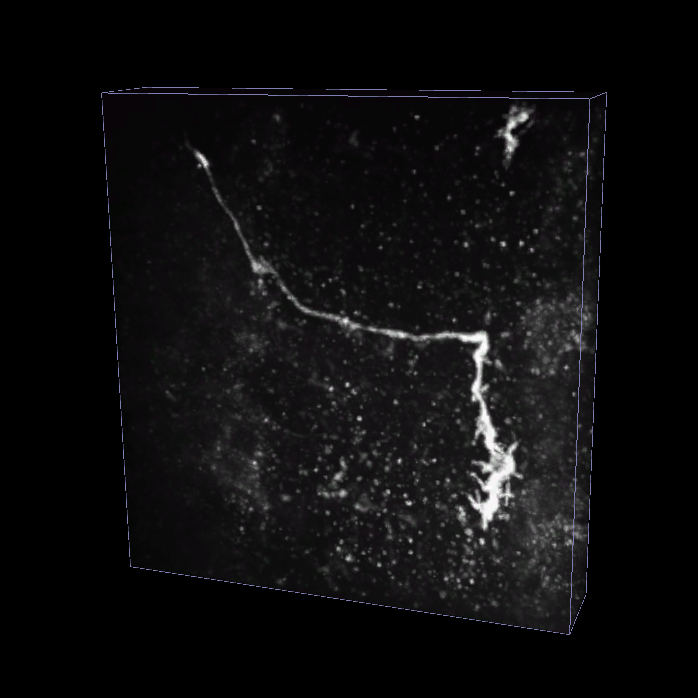
\includegraphics[width=0.29\textwidth]{images/lowSNR_1}	&
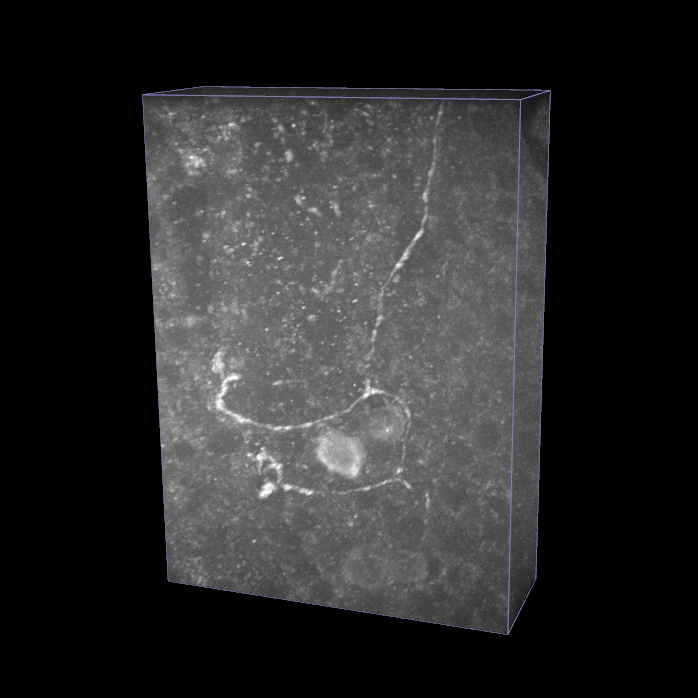
\includegraphics[width=0.29\textwidth]{images/lowSNR_2}	&
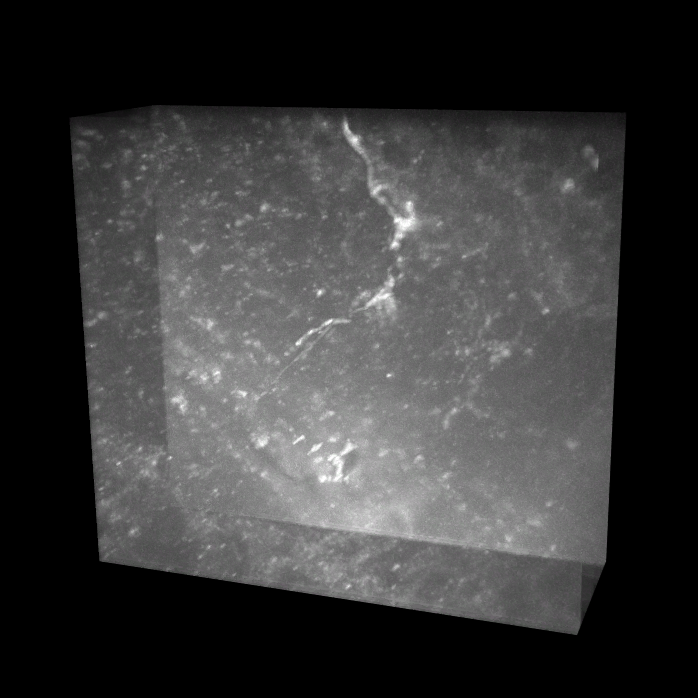
\includegraphics[width=0.29\textwidth]{images/lowSNR_3} \\
\scriptsize(a) & \scriptsize(b) & \scriptsize(c)
\end{tabular}
\caption[3D neuron example]{Drosophila neurons imaged by confocal microscope. (a) is a low SNR sensory neuron. The background clutter are due
to illuminated non neuronal filaments. (b) and (c) are interneurons, the image quality severely degraded by photon noise, low signal
intensity and in-homogeneous contrast.}
\label{fig:neuron_stack}
\end{figure}

We are interested in investigating the morphological properties of single neurons of the fruit fly Drosophila. A detailed survey of the imaging protocols is elaborate, and is out of scope of this dissertation. However, a brief summary of the imaging method is discussed here to understand on the dataset that we will be using for analyzing our algorithms.

Biologists have shown interest in studying the neuronal processes (axons, dendrites, synapses etc.) of the Drosophila, which has been a preferred model organism for to study genetics and developmental biology for several years.  The central nervous system (CNS) of the Drosophila contains a vast array of interacting synapses and neuronal processes in addition to containing about 20,000 neurons in the larval stage.  

Green Florescence Protein (GFP) is used to label the neuronal cells, which are produced through a combination of a FLP/FRT system and GAL4/UAS system. Approximately 10 hr old embryos were heat shocked at $37^\circ$C for 1-2 hrs, that generates single GFP-labeled cells \cite{barry_serotonergic}. Using this protocol, most Ventral Nerve Cord (VNC)'s have about 5 labeled cells, thus allowing for imaging of individual neurons.

For imaging the labeled cells, confocal microscopy was used to image the cells in three dimensions, with resolution in the micrometer range. Three images captured in the Condron Lab at the University of Virginia are shown in Fig.~\ref{fig:neuron_stack}





%\subsection{Neuron reconstruction posed as a vessel detection problem}
%
%As mentioned earlier, neurites are tubular structures which can be appropriately modeled as  tree shaped objects with varying degrees of branch bifurcations that determines its structural complexity. Several neuron reconstruction algorithms draw inspiration from the works in medical image analysis which focus on segmenting tubular or vascular objects from images. There have been a few methods proposed in the literature in this regard for different applications and modalities, such as segmentation of retinal blood vessels, human arteries from Computed Tomography Angiography images for detecting aneurysms \cite{gooya2012generalization,gooya2008variational,lesage2009review,shang2011vascular,nain2004vessel,jacob2004steerable,manniesing2006vessel,sofka2006retinal} etc.  Other non biomedical applications of vessel detection in the computer vision community include detection of tubular structures (such as roads, bridges etc.) from aerial images \cite{gonzalez_2010,turetken_MIP}, identifying cracks on concrete structures such as pavements and bridges \cite{oliveira2013automatic,crackd_TASE,oliveira2014crackit} etc. 
%
%However, despite the fact that the problem of vessel detection has been studied for quite some time, direct adaptation of an off-the-shelf algorithm to a particular task is still non trivial. This is due to the fact that each imaging application, with its associated modality pose different challenges in terms of denoising, object enhancement and clutter removal. For example, fluorescence microscopy images are often degraded by photon noise, inhomogeneous brightness of the objects and sporadic signal attenuation, which makes segmentation difficult. This requires an application specific approach that respects the local morphology of the structures, but is robust to the various imaging artifacts as well.  

\section{Contributions of this thesis}
The major emphasis of this dissertation will be on developing novel  algorithms for segmenting single neurons from confocal microscopy data. We realize that a large scale structural analysis of neuron groups demand efficient, automated segmentation to generate the digital morphology. Therefore, in this work, we primarily focus on developing and improving the first stepping stone for \textit{neuromics}-- automated neuron segmentation algorithms. 

%We start with a 2-d framework, and gradually progress to the more complicated 3-d segmentation problem. We identify the key issues which are necessary for robust neuron structure detection viz. prior enhancement of tubular neurites and the ability to deal with abrupt signal attenuation due to imaging artifacts. The segmentation algorithms are formulated so as to adequately respond to these issues. Finally, we propose a modification and improvement for the neuron enhancement step, which is an integral aspect for both the segmentation algorithms. We further show that the developed and proposed methodologies can also be used for a wide variety of applications which scale from bio-imaging to civil engineering. The specific aims of this dissertation are given below:
%
%\textit{The overall arrangement of the dissertation is as follows:
%
%\begin{itemize}
%\item \textbf{Chapter 1}: Introduction to the problem
%\item \textbf{Chapter 2}: Motivation and detailed background survey of segmentation of vascular structures, with an emphasis on neuron segmentation from confocal microscopy.
%\item \textbf{Chapter 3}: Motivation for using geometric active contours for seggmentation. Discussion of relevant level set based methodologies.
%\item \textbf{Chapter 4}: In this chapter we focus on neuron segmentation from 2D images and we propose a solution which tackles the inhomogeneity in the object illumination. 
%\item \textbf{Chapter 5}: In this chapter, we discuss our 3D neuron segmentation algorithm "Tubularity Flow Field (TuFF)". Qualitative and quantitative evaluation on a set of 3D confocal images  are presented. 
%\item \textbf{Chapter 6}: In this chapter, we propose a robust version of TuFF. This model incorporates a more suitable pre-processing step along with a component to reduce segmentation error due to contour leakage. A non biological application is discussed, which involves automated identification of cracks from concrete structures. 
%\item \textbf{Chapter 7}: Finally, in this chapter we conclude this thesis by discussing its salient features and identifying the future prospects. 
%\end{itemize}
%}

\subsubsection*{Contribution 1: Graph theoretic neuron segmentation}

We devise a novel neuron tracing technique Tree2Tree-2 \cite{mukherjee_T2T_2}, which combines the strengths of variational segmentation and graph based connectivity analysis of disjoint connected components. We also introduce a novel methodology to generate a \textit{medialness} function \cite{mukherjee_medialness} for tubular objects, for the purpose of obtaining a smooth tracing along the neuron centerline.

\subsubsection*{Contribution 2: Region based 2D segmentation with level sets}
2D analysis often serves as a preliminary step for understanding the anatomy of neurites. Furthermore, certain categories of neurons (e.g. sensory neurons on the cuticle layer of \textit{Drosophila} larva) are topologically flat and therefore, the third dimension of imaging does not yield useful information for analysis. In this regard, we have developed a general purpose segmentation algorithm which uses geometric active contours. The proposed algorithm, \textit{Legendre Level Set} (L2S)\cite{mukherjee_L2S} aims at segmenting the objects from microscopy images in presence of heterogeneous illumination. 

\subsubsection*{Contribution 3: Tubularity field based 3D segmentation with level sets}
We propose a novel neuron tracing architecture, Tubularity Flow Field (TuFF) \cite{mukherjee_TuFF}, which uses geometric active contours to perform segmentation guided by the local tubularity of the neurites. One advantage of using geometric active contours is that these techniques are adaptive to the topology of the objects. As a result, joining disjoint neurites can be handled in a natural framework unlike Tree2Tree-2, where error is often introduced in the solution due to improper connectivity handling. We also provide a mechanism to combat the sporadic signal loss across the structures by incorporating a specialized attraction force in our solution to merge nearby fragments. 

\section{Thesis outline}
The rest of the dissertation is organized as follows: In Chapter 2, we discuss popular neuron segmentation techniques, as well as relevant methodologies for pre-processing.  
The graph based segmentation algorithm is discussed in Chapter 3 and the results are scrutinized for both 2D and 3D data. We identify the pros and cons of our method and discuss the motivation of using geometric active contours for more flexibility in establishing component connectivity. 

In Chapter 4, a brief summary of geometric active contours is presented, followed by discussion of the proposed 2D segmentation method L2S in Chapter 5. The 3D segmentation case using TuFF is presented in Chapter 6, along with strategies to improve segmentation results using a robust non local vessel detection technique.  Finally, we conclude in Chapter 7 with discussion of the methods, their future extensions and possible applications.

Apart from the aforementioned primary contributions, we found that the developed algorithms are quite general, and have a wide variety of applications involving vascular structures. Two such applications are discussed in the Appendix; the first one involves segmenting human arteries from low SNR ultrasound imagery, and the second method relates to the civil engineering discipline, where the goal is to detect cracks in concrete structures such as bridges and pavements.

\section{Publications resulting from this work}

\textsc{Journal Publications}
\begin{itemize}
\item 
\textbf{S. Mukherjee}, B. Condron and S.T. Acton, "Tubularity Flow Field – A Technique For Automatic Neuron Segmentation," \textit{IEEE Transactions on Image Processing}, vol.24, no.1, pp.374,389, Jan. 2015

\item
\textbf{S. Mukherjee} and S.T. Acton, ``Region Based Segmentation in Presence of Intensity Inhomogeneity Using Legendre Polynomials," \textit{IEEE Signal Processing Letters}, vol.22, no.3, pp.298,302, March 2015

\item
R.Sarkar, \textbf{S. Mukherjee} and S.T. Acton, ``Dictionary Learning Level Sets" \textit{IEEE Signal Processing Letters} (\textit{under minor revision})

\item
\textbf{S. Mukherjee}, L. Boulton and S.T. Acton, "Concrete crack detection using edge assisted Tubularity Flow Field with local directional evidence", \textit{in preparation}.
\end{itemize}

\noindent \textsc{Conference Publications}
\begin{itemize}
\item
\textbf{S. Mukherjee} and S.T. Acton, ``Oriented Filters for Vessel Contrast Enhancement With Local Directional Evidence", \textit{IEEE ISBI 2015}(accepted).
\item
M. Consylman, \textbf{S. Mukherjee}, D.P. Mukherjee, B. Condron and Scott T. Acton, ``Social behavior analysis of Drosophila larvae via motion activity recognition", \textit{IEEE SSIAI 2014.}
\item
\textbf{S. Mukherjee}, B. Condron and S.T. Acton, ``Neuron segmentation with level sets", \textit{ACSSC 2013}:1078-1082
\item
R. Sarkar, \textbf{S. Mukherjee} and S. T. Acton, ``Shape descriptors based on compressed sensing with application to neuron matching", \textit{ACSSC 2013}: 970-974
\item
\textbf{S. Mukherjee} and S. T. Acton, ``Vector field convolution medialness applied to neuron tracing," \textit{ICIP 2013}: 665-669
\item
\textbf{S. Mukherjee}, B. Condron and S. T. Acton, ``Chasing the neurome: Segmentation and comparison of neurons," \textit{EUSIPCO 2013}: 1-4
\item
\textbf{S. Mukherjee}, S. Basu, B. Condron and S.T. Acton , ``Tree2Tree2: Neuron tracing in 3D," \textit{ISBI 2013}: 448-451
\item
\textbf{S. Mukherjee}, S. Basu, B. Condron and S.T. Acton, ``A geometric-statistical approach toward neuron matching", \textit{ISBI 2012}: 772-775.

\end{itemize}

%\subsubsection*{Aim 1: Algorithm for neuron segmentation in 2D}
%
%Our first goal is to develop a generalized segmentation policy for  2D microscopy images. 2D analysis often serves as a preliminary step for understanding the anatomy of neurites. Furthermore, certain categories of neurons (e.g. sensory neurons on the cuticle layer of \textit{Drosophila} larva) are topologically flat and therefore, the third dimension of imaging does not yield useful information for analysis. 
%
%In this regard, we have developed a general purpose segmentation algorithm which uses geometric active contours. The proposed algorithm, \textit{Legendre Level Set} (L2S) aims at segmenting the objects from microscopy images in presence of heterogeneous illumination. We also briefly discuss a closely related algorithm \textit{Dictionary Learning Level Set}, which uses dictionary learning to tackle the intensity inhomogeneity. 
%
%\subsubsection*{Aim 2: Algorithm for neuron segmentation in 3D}
%Morphological characteristics of a vast majority of neurons are better captured using 3D imaging. A vast majority 3D images of the Green Fluorescence Protein (GFP) stained adult \textit{Drosophila} fruit fly is obtained at the Dept. of Biology, University of Virginia using confocal microscope. The GFP is expressed in single neurons using a heat shot activated scheme, which allows imaging at the single cell resolution\cite{barry_branching}.
%
%First, we discuss a graph theoretic segmentation algorithm \textit{Tree2Tree-2}, where the idea is to treat the neuron connectivity analysis problem using graph based algorithms. Details of Tree2Tree-2 are presented in Chapter 2. The second method, \textit{Tubularity Flow Field} or TuFF uses geometric active contours to perform segmentation guided by the local tubularity of the neurites. One advantage of using geometric active contours is that these techniques are adaptive to the topology of the objects. As a result, joining disjoint neurites can be handled in a natural framework unlike Tree2Tree-2, where error is often introduced in the solution due to improper connectivity handling. We also provide a mechanism to combat the sporadic signal loss across the structures by incorporating a specialized attraction force in our solution to merge nearby fragments. 
%
%\subsubsection*{Aim 3: Robust TuFF and other applications}
%
%Tubularity Flow Field is an effective mode of segmenting vascular shapes both in 2D and 3D applications. However, there are some aspects of TuFF which limits its broad applicability. To address these needs, we discuss a robust algorithm known as \textit{Edge Assisted TuFF} or EATuFF. The major highlights of EATuFF over TuFF is the addition of a specialized preprocessing step called Local Directional Evidence (LDE) which uses non local steerable filters to identify tubular structures in low contrast imagery. Second, an edge based attraction term is associated with the TuFF segmentation framework to reduce the contour leakage phenomenon which may occur if the image contrast is low. 
%
%We further demonstrate the applicability of our algorithm for a non biological application which involves detecting cracks on concrete structures. Although the application differs significantly from microscopy, these cracks can also be modeled as tubular objects. We show that EATuFF can be efficiently applied for this application with promising results.

